\documentclass[aspectratio=169]{beamer}
\input{preamble-update.tex}
\usepackage[compat=1.0.0]{tikz-feynman}
\title[HPS Analysis Workshop]{iDM and Me}
\begin{document}

\begin{frame}
  \maketitle
\end{frame}

\begin{frame}{Me}
  \begin{itemize}
    \item 5th Year Graduate Student at UMN
    \item Deeply integrated into LDMX collaboration
    \item Excited to learn with and about a sibling project
  \end{itemize}
  \vfill
  \begin{block}{Expertise}
    {\color{UMNMaroon}Software}, specifically containers, C++, Python, Geant4, and ROOT
  \end{block}
\end{frame}

\begin{frame}{Me}{HPS Projects}
  \begin{block}{Three Prong Tridents}
    with {\color{UMNMaroon}Cam} as {\color{UMNGold}Service} \\
    Developing analysis in \code{hpstr} to hopefully have a clean measurement of tracking efficiency
  \end{block}
  \begin{block}{Tracker Alignment via Kalman Tracks}
    with {\color{UMNMaroon}PF} as {\color{UMNGold}Service} \\
    Studying why Kalman tracks refit with GBL do not behave the same as original GBL tracks
  \end{block}
  \begin{block}{2016 iDM}
    with {\color{UMNMaroon}???} as {\color{UMNGold}Analysis} \\
    Analyze 2016 physics run, similar to SIMP search but studying differences carefully
  \end{block}
\end{frame}

\sectionframe{Three Prong Tridents}

\begin{frame}{Status}
  \begin{itemize}
    \item Familiarized with \code{hpstr} \checkmark
    \item Developed a pretty clean-cut analysis focused on finding ``clean" track events
  \end{itemize}
  \begin{columns}
    \begin{column}{0.5\textwidth}
      \begin{figure}
        \centering
        \includegraphics[width=0.7\textwidth]{figs/pos_cluster_E_sum.pdf}
      \end{figure}
    \end{column}
    \begin{column}{0.5\textwidth}
      \begin{figure}
        \centering
        \includegraphics[width=0.7\textwidth]{figs/pos_electron1_track_N.pdf}
      \end{figure}
    \end{column}
  \end{columns}
\end{frame}

\begin{frame}{Plans}
  \begin{itemize}
    \item Generalize analysis
      \begin{itemize}
        \item Show ECal crystal occupancy
        \item Include dead/off crystals as part of ``the edge" when determining if clusters are fiducial
        \item Check trigger clusters (for runs where that data was saved)
      \end{itemize}
    \item Merge processor and its configuration JSONs
  \end{itemize}
\end{frame}

\sectionframe{Tracker Alignment}

\begin{frame}{Status}
  \begin{itemize}
    \item Met with HPS folks (PF, Norman, Robert) \checkmark
    \item Running \code{hps-java} with PF \checkmark
    \item Learning about alignment and tracking procedures
      \footnote{Shoutout to PF for being a great tutor}
  \end{itemize}
  \begin{figure}
    \centering
    \includegraphics[width=0.4\textwidth]{figs/gbl_kf_chi2.png}
  \end{figure}
\end{frame}

\begin{frame}{Plans}
  \begin{itemize}
    \item Introduce known misalignment and try to re-align
    \item Search for difference between KF and GBL alignment procedures
  \end{itemize}
\end{frame}

\sectionframe{2016 iDM}

\begin{frame}{Status}
  \vfill
  \centering
  \begin{beamercolorbox}[sep=8pt,center,shadow=true,rounded=true]{title}
      \usebeamerfont{title}noop\par%
  \end{beamercolorbox}
  \vfill
\end{frame}

\begin{frame}{Status}
  \begin{figure}
    \centering
    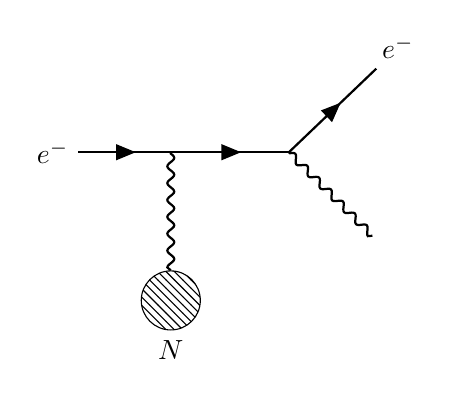
\begin{tikzpicture}
      \begin{feynman}
        \vertex (a) {$e^{-}$};
        \vertex [right= of a](d);
        \vertex [below=of d, blob,label={below:$N$}] (e) {};
        \vertex [above right= of d] (f);
        %\vertex [above right= of d] (b);
        \vertex [right= of d] (b);
        \vertex [above right= of b] (g) {$e^{-}$};
        \vertex [below right= of b] (h) {\aprime};
        \diagram*[large] {
          (a) -- [fermion] (d),
          (d) -- [boson] (e),
          (d) -- [fermion] (b),
          (b) -- [fermion] (g),
          (b) -- [boson] (h),
        };
      \end{feynman}
    \end{tikzpicture}
  \end{figure}
\end{frame}

\begin{frame}{Plans}
  \begin{itemize}
    \item Develop {\sc MadGraph} model with help from theorists
    \item Put model into HPS and see how this signal behaves differently than SIMPs
    \item Cut-n-count analysis of 2016 physics data
  \end{itemize}
\end{frame}

\end{document} 
